\chapter[FM - Modulateion and Demodulation using PLL]{FM - Modulateion and Demodulation using PLL}
\section*{Aim}
To implement FM modulation and demodulation circuits using PLL IC CD4046
\section*{Theory}
CD 4046 is an analog Phase Locked Loop IC, whose characteristics and features are discussed in Appendix \ref{4046}. 
\subsection*{FM Modulation}

The VCO part of the PLL may be used for the frequency modulation of the carrier. In a VCO, the output frequency is proportional to the control volatge input. In the absance of control voltage, the free running frequency is determined by the supply voltage $V_{CC}$, the externally connected resistances $R_1$ and $R_2$ and the capacitance C. The free running frequency $f_0$ is given by 
\begin{equation}
f_0=\frac{0.16\ X\ \frac{V_{CC}}{2} }{R_1.C}+\frac{1}{R_2.C}
\end{equation}

This is the carrier for FM generator. The control input, pin-9 is clamped at a voltage $\frac{V_{cc}}{2}$. The modulating signal voltage which is less than 2.5V, -\emph{say 1 $V_{pp}$}and frequency 1 kHz is applied at pin-9 through a capacitor.

\subsection*{FM Demodulation}
Another PLL IC has to be used for FM demodulation. The VCO part of this IC is configured for the same free running frequency as that of the modulator IC. 

The modulated signal is applied to voltage signal input of the phase detector, the pin-14. The other input of the phase detector- \emph{pin 3}- is fed with the VCO output- \emph{pin 4}. 

 The demodulated output will be obtained at the emitter of internal emitter follower by pulling down the pin to ground through a resistor. This demodulated output contains ripples which may be removed using a lowpass filter.
\section*{Design}
\section*{Circuit Diagram}
\begin{figure}
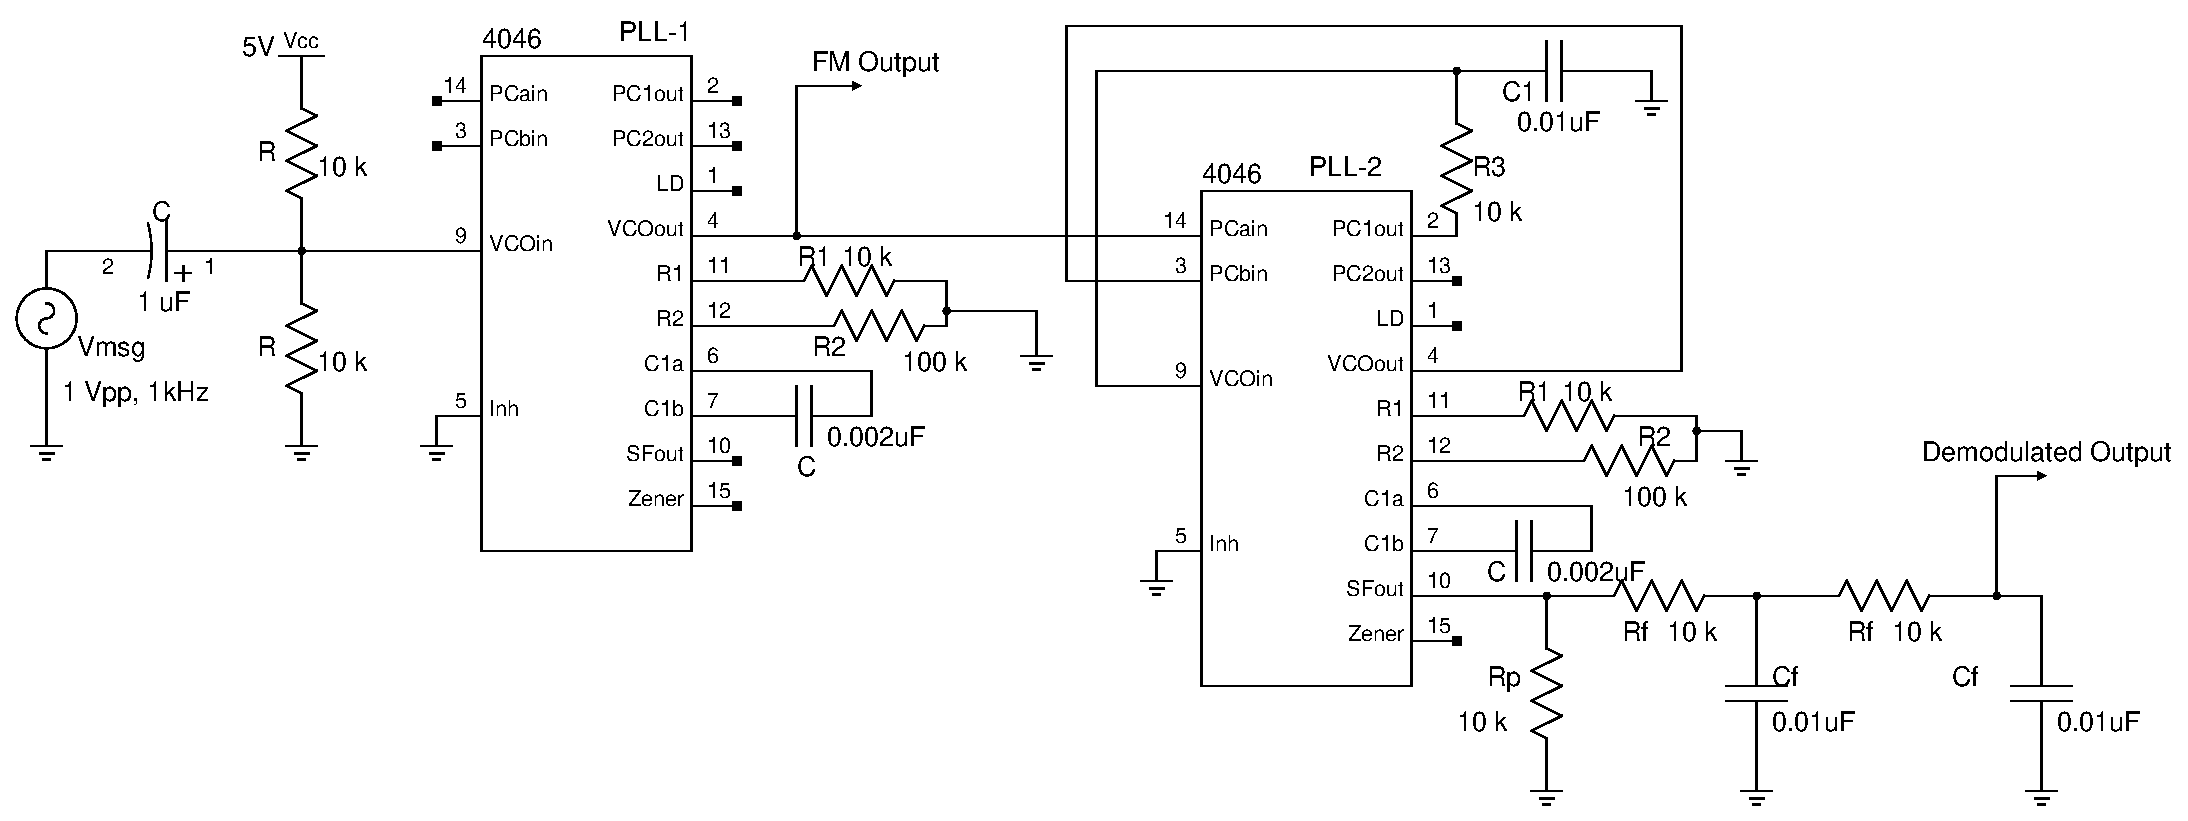
\includegraphics{fmpll.eps}

\end{figure}

\section*{Procedure}
\section*{Observation}
\section*{Result}
